\subsection{The current state of ECDAR} %This was written quite fastly ;)
To further illustrate what ECDAR is, and how far its been developed. 
We will go through the tool in this section, a screenshot of which can be found in figure \ref{fig:ECDAR-gui}. 
The version of ECDAR displayed and described here is ECDAR version 2.3.3 from 2022-09-08 downloaded from \href{https://www.ecdar.net/download/}{www.ecdar.net/download/}.

\begin{figure}[H]
    \centering
    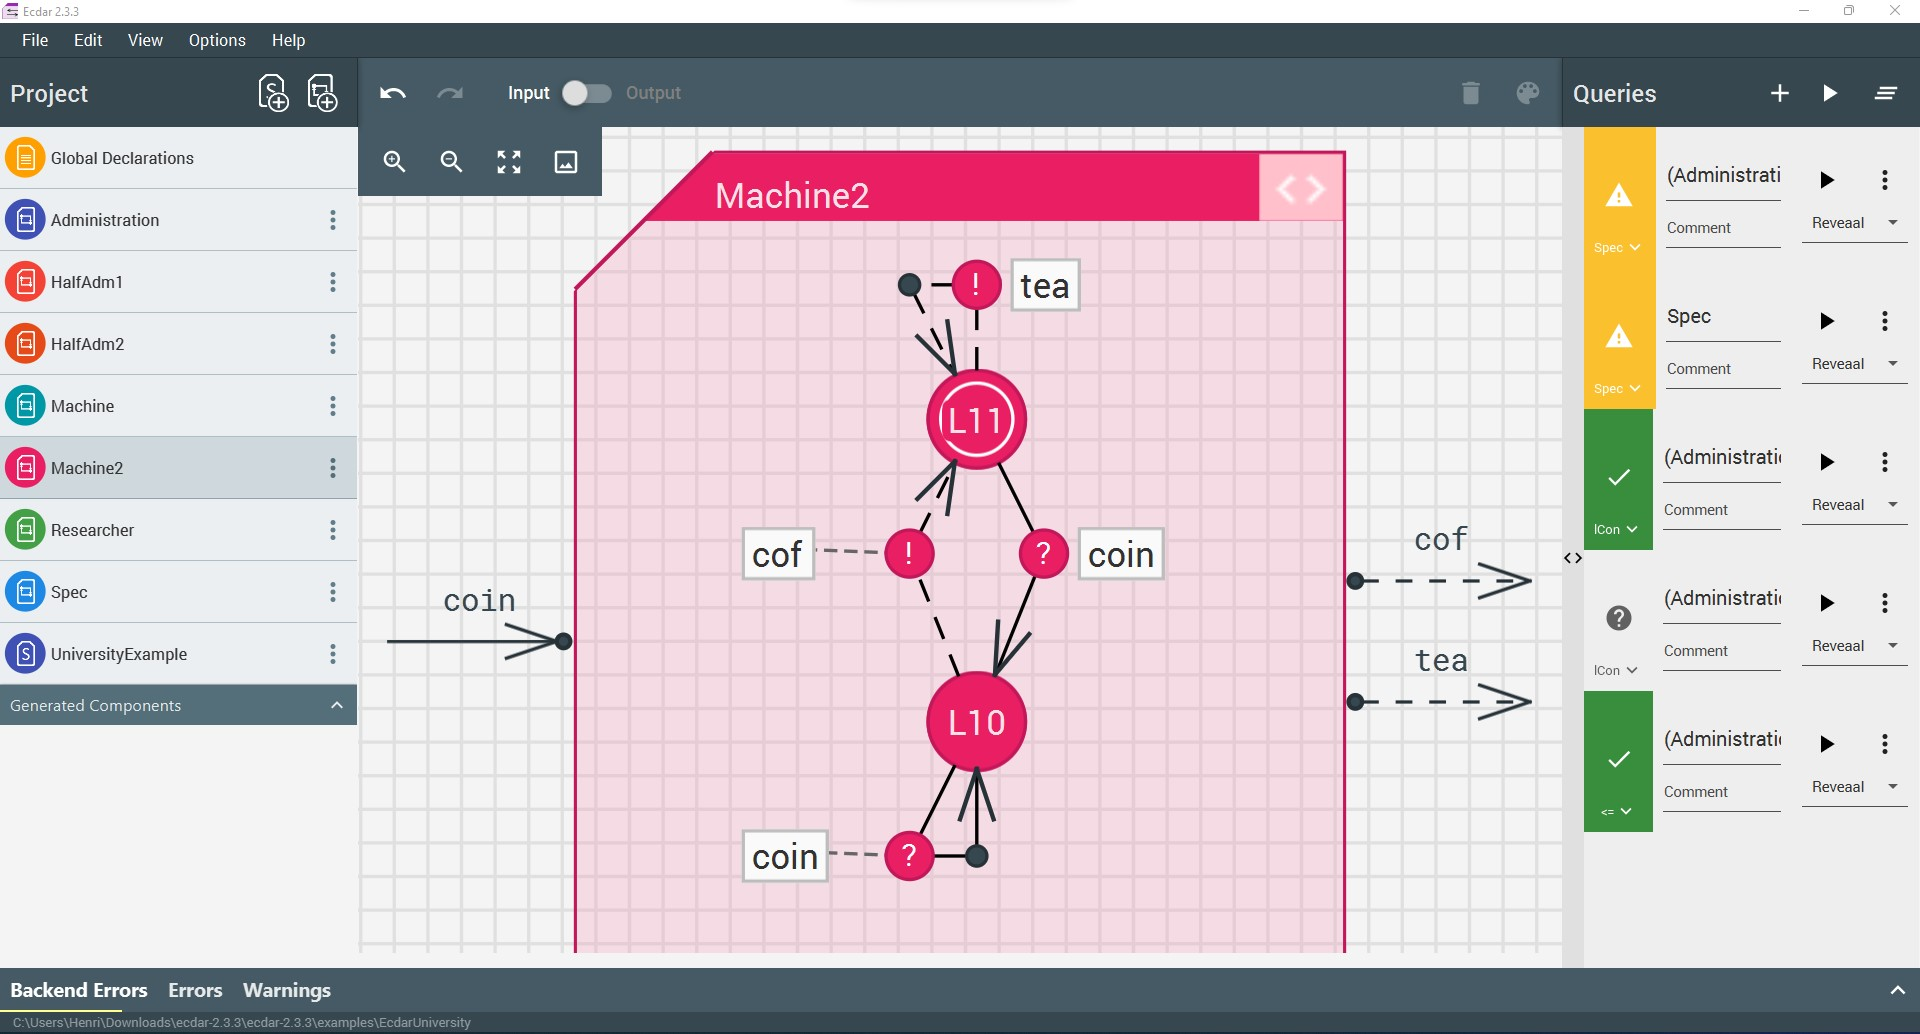
\includegraphics[width=1\textwidth]{common/figures/ecdar-overview.jpg}
    \caption{A screenshot of the ECDAR GUI.}
    \label{fig:ECDAR-gui}
\end{figure}
The top bar of the GUI has five tabs, the leftmost being \textit{File}, this is used to open, save and create new projects.
The other tabs are self explanatory.
Positioned right underneath the \textit{Help} tab are the two buttons for creating new models and new specifications.

The panel on the left contains an overview of the components and specifications. 
In this panel the component \textit{Machine2} is selected which is displayed in the middle of the GUI.
ECDAR allows the user to create a type of automata called \textbf{T}imed \textbf{I}nput \textbf{O}utput \textbf{A}utomata. 
This automaton takes \texttt{coin} as input, since the arrow is solid, and the automaton outputs \texttt{cof} and \texttt{tea}, as shown by the dashed arrows on the left side of the automaton.
Inside the red box the \texttt{L11} location is marked as the start state, which is indicated by the circle.
A solid arrow through a small circle with a question mark represent an output. 
Likewise, if the arrow is dashed and the small circle contains an exclamation mark, it represents an input.
This concludes the possibilities regarding input and output.

Figure \ref{fig:ECDAR-guard} contains an automaton which uses time as well as input and output.
This is done by using a clock, which is represented as the variable y.
\begin{figure}[H]
    \centering
    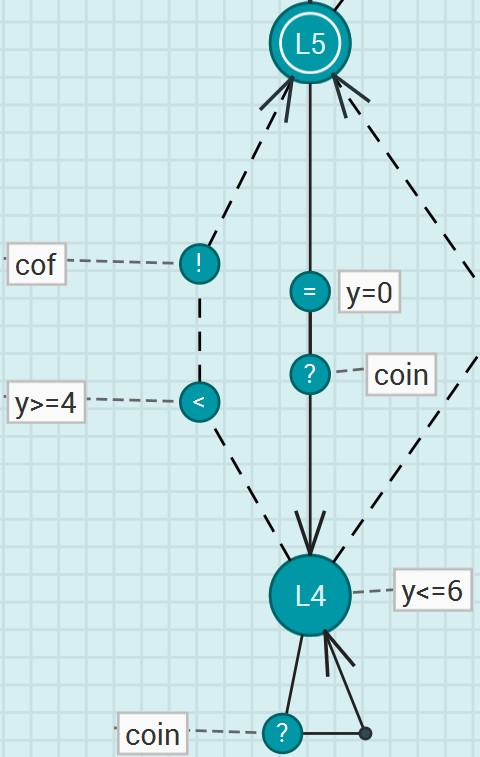
\includegraphics[width=0.3\textwidth]{common/figures/ecdar-guards.jpg}
    \caption{A screenshot of an automaton with a guard and an invariant.}
    \label{fig:ECDAR-guard}
\end{figure}
The transition with the small circle containing the assignment is an \textit{update}, which resets the clock.
The small circle containing a less then sign is a \textit{guard}, which can be thought of as a restriction, which must be satisfied in order to take this action/transition.
Finally the \texttt{L4} location contains an \textit{invariant} \texttt{y<=6}, which must be satisfied. 
In this case it means the automaton cannot be in the location, if the clock value exceeds the value 6.
The mechanics of TIOAs will be elaborated in \ref{subsub:automata}.

The rightmost panel with queries 

different checks

syntax of the field like: m2 || m2 $<=$ spec

option to choose different engines



